%%%%%%%%%%%%%%%%%%%%%%%%%%%%%%%%%%%%%%%%%
% Stylish Article
% LaTeX Template
% Version 2.1 (1/10/15)
%
% This template has been downloaded from:
% http://www.LaTeXTemplates.com
%
% Original author:
% Mathias Legrand (legrand.mathias@gmail.com)
% With extensive modifications by:
% Vel (vel@latextemplates.com)
%
% License:
% CC BY-NC-SA 3.0 (http://creativecommons.org/licenses/by-nc-sa/3.0/)
%
%%%%%%%%%%%%%%%%%%%%%%%%%%%%%%%%%%%%%%%%%

%----------------------------------------------------------------------------------------
%	PACKAGES AND OTHER DOCUMENT CONFIGURATIONS
%----------------------------------------------------------------------------------------

\documentclass[fleqn,10pt]{SelfArx} % Document font size and equations flushed left
\usepackage{fontspec}
\usepackage[english]{babel} % Specify a different language here - english by default

\usepackage{lipsum} % Required to insert dummy text. To be removed otherwise
\usepackage{float}
\usepackage{listings}

% ----------------------------------------------------------------------------------------
%	COLUMNS
%----------------------------------------------------------------------------------------

\setlength{\columnsep}{0.55cm} % Distance between the two columns of text
\setlength{\fboxrule}{0.75pt} % Width of the border around the abstract

%----------------------------------------------------------------------------------------
%	COLORS
%----------------------------------------------------------------------------------------

\definecolor{color1}{RGB}{0,0,180} % Color of the article title and sections
\definecolor{color2}{RGB}{0,20,20} % Color of the boxes behind the abstract and headings
\definecolor{color3}{RGB}{0,180,90} % Color of the boxes behind the abstract and headings

%----------------------------------------------------------------------------------------
%	HYPERLINKS
%----------------------------------------------------------------------------------------

\usepackage{hyperref} % Required for hyperlinks
\hypersetup{hidelinks,colorlinks=true,breaklinks=true,urlcolor=color3,citecolor=color1,linkcolor=color1,bookmarksopen=false,pdftitle={Title},pdfauthor={Author}}

%----------------------------------------------------------------------------------------
%	ARTICLE INFORMATION
%----------------------------------------------------------------------------------------

\JournalInfo{CS-E3210 Data Analysis Project} % Journal information
\Archive{Aalto University} % Additional notes (e.g. copyright, DOI, review/research article)

\PaperTitle{Comparison of learning models for music genre classification} % Article title

\Authors{} % Student\textsuperscript{1}, Student\textsuperscript{2}} % Authors
\affiliation{\textsuperscript{1}\textit{}} % Author affiliation
\affiliation{\textsuperscript{2}\textit{}} % Author affiliation
%\affiliation{\textbf{Corresponding author}: john@smith.com} % Corresponding author

\Keywords{Keyword1 --- Keyword2 --- Keyword3} % Keywords - if you don't want any simply remove all the text between the curly brackets
\newcommand{\keywordname}{Keywords} % Defines the keywords heading name

%----------------------------------------------------------------------------------------
%	ABSTRACT
%----------------------------------------------------------------------------------------

\Abstract{\lipsum[1]~}

%----------------------------------------------------------------------------------------

\begin{document}
  \boldmath

\flushbottom % Makes all text pages the same height

\maketitle % Print the title and abstract box

\tableofcontents % Print the contents section

\thispagestyle{empty} % Removes page numbering from the first page

%----------------------------------------------------------------------------------------
%	ARTICLE CONTENTS
%----------------------------------------------------------------------------------------

\phantomsection
\section{Introduction} % The \section*{} command stops section numbering

%\addcontentsline{toc}{section}{Introduction} % Adds this section to the table of contents

\lipsum[1-3] % Dummy text

%------------------------------------------------

\section{Data Analysis}

Before diving deep into applying some machine learning algorithms it is useful
to explore the data a bit to get a general idea of the features and quirks of
the data set. Our data analysis process began by printing the values for some randomly
selected data points. The raw data does not make much sense and it is
challenging to try to find some correlation between certain classes and some
selected features. However, in that small sample a disproportionate share of the
labels were \textit{Pop\_Rock} or class $1$. The next logical step was to take a
closer look at the class distribution of the given data and see if the observed
unbalanced distribution is just randomness or a feature of the data set. The
class distribution has been visualized in figure \ref{fig:dist-hist} and the
dominance of class $1$ can be clearly seen. This imbalance might be due to
having two popular music generes, pop and rock, under one label but it can also
be just a feature of the data set.
% TODO: is is appropriate to discuss generalization of the class distribution here?
Intuitively the disproportionate class distribution makes sense but for
practical applications that have to work on any unlabeled data set, any
assumptions can hardly be made.

\begin{figure}[H]
  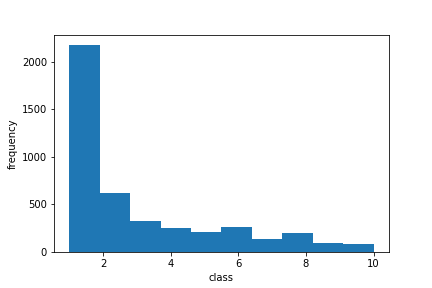
\includegraphics[width=\linewidth]{class-dist-hist.png}
  \caption{Distribution of classes in the data set}
  \label{fig:dist-hist}
\end{figure}

Another interesting feature of the data set is the low number of samples with
relation to the amount of features. Since there are 4363 songs and each of them
have 264 features, it is obvious that the dataset is nowhere near sufficient to
explore all combinations of all features. Most likely the whole space is not
needed to represent all common music generes but in spite of this, the size of
the data set might be the limiting factor. We could overcome this by finding a
subset of the original features that preserve the information of 264 features.
Since the feature space includes multiple statistics of rhythm and chroma, there
could be some correlation that could be exploited to reduce the dimensionality.
The correlation heatmap for the training data in figure \ref{fig:heatmap} shows
that there is indeed some correlation and especially the seven rhythm statistics
are nicely separable.

\begin{figure}[H]
  \centering
  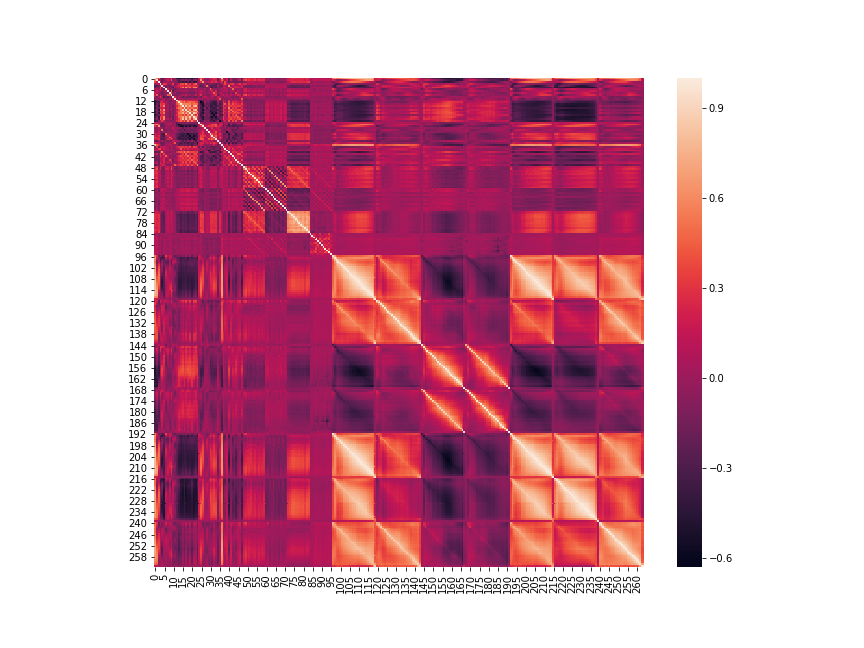
\includegraphics[width=\linewidth]{heatmap.png}
  \caption{Correlation heatmap}
  \label{fig:heatmap}
\end{figure}

The heatmap is a nice visualization but it would be hard to manually engineer a
new feature space that captures the details that matter. For the actual
dimensionality reduction task principal component analysis is a much better
candidate.
% TODO: should we have some reference to PCA details/implementation here?
The variance explained by PCA is illustrated in figure \ref{fig:pca}. The figure
suggests that the first few principal components explains the majority of the
variance and with 10 principal components almost all the variance is explained.
The heatmap also indicates that there could be some redundant
features so a more interpretable dimensionality reduction technique would be to
just discard features that do not have sufficient contribution to the total variance.

\begin{figure}[H]
  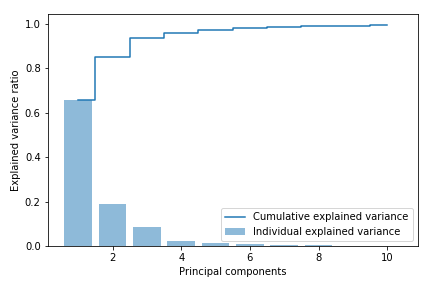
\includegraphics[width=\linewidth]{pca.png}
  \caption{Variance explained by principal components}
  \label{fig:pca}
\end{figure}


\section{Methods and Experiments} % The \section*{} command stops section numbering

In order to experiment with different ideas and approaches it is important to
set up a machine learning pipeline. Such pipeline should take the raw data as input and produce
an accurate description of the quality of the underlying classifier and the
classification output when desired. Ideally this pipeline can easily be used to
test different classifiers and also to find sufficient hyperparameters for them.
Another desirable qualities are speed and accurate estimations of the
performance. This section describes how we set up our pipeline and what were the
most promising approaches we came up with.

\subsection{Pipeline and evaluation methodology}

We used pandas framework to read and write the csv-files and relied
heavily on scikit-learn to build a robust machine learning pipeline that could
effortlessly be used to try different preprocessing steps and machine learning
algorithms with sufficient hyperparameters. An example of such pipeline using
logistic regression classifier is provided in appendix \ref{sklearn-example}
% TODO: add code to appendix and refer to it

As was mentioned in the previous section, the set of labeled data points is
relatively small when considering the classification task. Therefore we decided
to use cross-validation instead of a separate validation set. To be more
specific, we used stratified k-fold that takes into account the
unbalanced class weights. There is no single configuration which we used since we
had to do some modifications in order to find the right balance between variance
and performance. One of these configurations, for example, was to use 5x3
cross-validation where the data was split into five folds and then the data of
the four training
folds was once again split into three folds out of which two were used to train the
model and one was used to optimize the hyperparameters. This approach resulted
in good hyperparameter values and an accurate estimation of the performance.

All in all, our pipeline consists of reading the csv file, splitting the data into
appropriate training and validation sets, standardizing the data, possibly reducing
the dimensionality and then training and tuning a classifier. The tuned
classifier is then either described by some performance metrics or it is used to
label the unlabeled data. We relied heavily on this pipeline to evaluate the
performance of a classifier instead of submitting the results of every
prominent classifier to the Kaggle competition. As a result we might have
overlooked some classifier that has been rated against an undesirable or
unrepresentative validation set. However, this approach is more likely to work
with a real-life machine learning problem.

\subsection{Algorithms and methods}

% TODO: List the following algos/methods as subsubsections?

%\addcontentsline{toc}{section}{Methods and Experiments} % Adds this section to the table of contents
\underline{Fundamental intuition for choosing models:} Multi-class classification being the underlying aspect of the problem statement, we turned to learning models which constitute this feature.

\subsection{Logistic Regression}~\\
\underline{Motivation:} Logistic regression though by nature the default for binary classification, the fact that it can be extended for multi-class models was the motivation for choosing it.

Our model predicted the probabilities of different possible genres (labels) corresponding to a given feature space (see the data analysis section). For each of the multi-classification modelling techniques [one-vs-one - $ovo$, one-vs-all - $ovr$], we empirically used various algorithms as solvers (like stochastic average gradient) and consecutively varied the following parameters.
\begin{itemize}
  \item Maximum iterations for convergence ($100-900$)
  \item Initial class weights (balanced weighing, initializing to $1$)
  \item Weight regularization strength ($0.1-0.9$)
  \item Tolerance of error across runs
\end{itemize}
in focus of improving on the accuracy of and reducing loss of the classification.

To optimize the hyper-parameters for modelling the logistic regression classifier we made use of the exhaustive Grid-search cross validation technique.

\subsection{Support Vector Machines}~\\
\underline{Motivation:} As the feature-space is of a relatively higher dimensionality, we decided to try out support vector machines to improve on the statistics achieved using the logistic model.

Initially, we modelled a linear support vector classifier which used set of hyperplanes for learning the training data. As we did not observe any drastic improvements in the statistics, we further analysed the data and decided to experiment with the non-linear modelling of the support vector machines.

While empirically using both $ovo$ and the $ovr$ techniques, we tested various kernels:
\begin{itemize}
  \item Gaussian radial basis function
  \item Polynomial (degree 3)
  \item Sigmoid
\end{itemize}

For each of the kernels we varied the following parameters:
\begin{itemize}
  \item Maximum iterations for convergence ($100-300$)
  \item Initial class weights (balanced weighing, initializing to $1$)
  \item Weight regularization strength ($0.1-0.9$)
  \item Tolerance of error across runs
\end{itemize}

To optimize the hyper-parameters for modelling the support vector classifier we made use of the exhaustive Grid-search cross validation technique.
\subsection{Ensemble Classifier}~\\
\underline{Motivation:} After experimenting with the above two models for sometime, we figured that logistic regression classifiers were good with accuracy metric and SVMs were minimizing on the log-loss statistic. So we decided to ensemble them together to understand if we can get the better of both worlds.

We used the \textbf{voting classifier} strategy to combine the above classifiers using a majority vote to predict the genres. We used both hard and the average predicted probabilities voting (soft vote) methods and found that the hard voting produced better results.

\subsection{Semi-Supervised Classifier}~\\

\underline{Motivation:} After not being able to further deduce any meaningful direct relationship between the feature-space, we decided to try the semi-supervised learning methodology.

We chose the label-spreading strategy over label propagation as it is more robust to noise{\cite{label-spreading}}. Modelling steps:
\begin{itemize}
  \item[\textit{Step 1}] Splitting the labelled (train) data as based on some percentage (we chose $\frac{1}{3}^{rd}$ of the it for validation)
  \item[\textit{Step 2}] Merging the split of labelled data from [step-1] with the unlabelled data.
  \item[\textit{Step 3}] Training the classifier/kernel chosen for label-spreading with respective parameters (listed below)
  \item[\textit{Step 4}] Scoring/validating the trained model using the split test data from [step-1]
  \item[\textit{Step 5}] Predicting the genres for unlabelled (actual test) data
\end{itemize}

We varied the following parameters over runs:
\begin{itemize}
  \item Kernels ($rbf$, k-nearest neighbours). Varying the gamma parameter (b/w $0.1-00001$) and the number of neighbours attribute (b/w $50-300$) respectively.
  \item Maximum iterations for convergence ($100-300$)
\end{itemize}

\subsection*{Other models}~\\
Apart from the above mentioned classifiers, we experimented with more models that did not pass our benchmarks for both the accuracy and loss metrics.
\begin{itemize}
  \item Naive Bayes'
  \item Decision trees
  \item Random forests
\end{itemize}

Though we initially considered reducing the dimensionality by performing principal component analysis, after some substantial scrutiny of the feature space we dropped it. The rhythm bands, pitch classes and the timbre coefficients we spread out across the statistics to discard.

\subsection*{Performance Metrics}~\\
Evaluation of all the models designed was done using the $k$-fold cross validation technique (with $k=5$).

For splitting the data into folds we used stratified process of preserving the percentage of samples for each genre thereby enabling fair evaluation.
%------------------------------------------------

%------------------------------------------------


\section{Results}

Performance measures of the above experiments when evaluated with the test data.

\subsection{Accuracy, Log-Loss statistics}
\begin{itemize}
  \item Logistic Regression Classifier across various values for its parameters. Results for the best 5 combinations:
  \begin{table}[H]
    \caption{metrics on test data (LR)}
    \centering
    \begin{tabular}{llrr}
      \toprule
%			\multicolumn{2}{c}{Name} \\
%			\cmidrule(r){1-2}
      modelling strategy & solver & accuracy & loss \\
      \midrule
      ovr & sag & $0.658$ & $0.12$ \\
      multinomial & sag & $0.653$ & $0.17$ \\
      ovr & liblinear & $0.650$ & $0.21$ \\
      ovr & lbfgs & $0.646$ & $0.26$ \\
      ovr & newton-cg & $0.646$ & $0.26$ \\
      \bottomrule
    \end{tabular}
    \label{tab:label}
  \end{table}
  \item Support vector classifiers across various values for its parameters. Results for the best 5 combinations:
  \begin{table}[H]
    \caption{metrics on test data (SVC)}
    \centering
    \begin{tabular}{llrr}
      \toprule
      %			\multicolumn{2}{c}{Name} \\
      %			\cmidrule(r){1-2}
      modelling strategy & kernel & accuracy & loss \\
      \midrule
      multinomial & rbf & $0.636$ & $0.07$ \\
      ovr & rbf & $0.636$ & $0.07$ \\
      multinomial & linear & $0.607$ & $0.20$ \\
      ovr & linear & $0.607$ & $0.20$ \\
      ovr & poly (degree 3) & $0.567$ & $0.36$ \\
      \bottomrule
    \end{tabular}
    \label{tab:label}
  \end{table}
  \item Ensemble classifier with best parametric combination of logistic regression, SVC and voting strategy produces
  $$accuracy = 0.631, loss = 0.09$$
  \item Semi-supervised classifier with label spreading:
  \begin{table}[H]
    \caption{metrics on test data (semi-supervised)}
    \centering
    \begin{tabular}{llrr}
      \toprule
      %			\multicolumn{2}{c}{Name} \\
      %			\cmidrule(r){1-2}
      kernel & attribute & accuracy & loss\\
      \midrule
      knn & neighbours(300) & $0.533$ & $0.14$ \\
      rbf & $\gamma=0.001$ & $0.612$ & $0.29$ \\
      \bottomrule
    \end{tabular}
    \label{tab:label}
  \end{table}
\end{itemize}

\subsection{Confusion matrix}
The following confusion matrix represents the accuracy of classification. It is evident that the prediction is directly influenced by the frequency of respective genres in the training data.
\begin{figure}[H]
  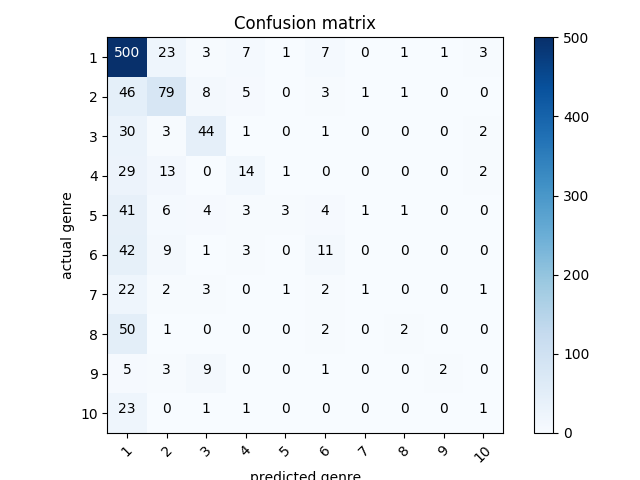
\includegraphics[width=\linewidth]{confusion-matrix.jpg}
\end{figure}

The matrix entry $i$, $j$ is the number of songs actually in genre $i$, but predicted to be genre $j$. Darker the blue, accurate the classification.

\section{Discussion}

%----------------------------------------------------------------------------------------

\section{Appendices}
% TODO: for appendix and reference list we don't want two columns
% also there is \appendix, is it more appropriate?

\subsection{Pipeline using scikit-learn} \label{sklearn-example}

The following code snippet illustrates how easy it is to set up a machine
learning pipeline in scikit-learn assuming \textit{load\_data} is a function that
loads the data set. \textit{LogisticRegressionCV} is a class that trains a
logistic regression classifier using all the listed C-values and uses the
best-performing classifier to calculate accuracy on the test set. A similar
class that can be used to optimize hyperparameters in scikit-learn is
\textit{GridSearchCV} \cite{gridsearchcv}.

\lstinputlisting[language=Python]{pipeline.py}

%----------------------------------------------------------------------------------------
%	REFERENCE LIST
%----------------------------------------------------------------------------------------

\phantomsection
\begin{thebibliography}{2}
  % TODO: I would say it is better to have plaintext links instead of href
  % anyways let's make these consistent before submitting
  % (see todo about making appendix and references normal 1 column page)

\bibitem{label-spreading}
  \href{http://scikit-learn.org/stable/modules/generated/sklearn.semi\_supervised.LabelSpreading.html}{semi-supervised learning,}

\bibitem{gridsearchcv}
  \textit{GridSearchCV}, \\
  \texttt{http://scikit-learn.org/stable/modules/generated/sklearn.model\_selection.GridSearchCV.html}
\end{thebibliography}

%----------------------------------------------------------------------------------------


\end{document}